\documentclass[letterpaper,11pt]{article}
\usepackage{graphicx}
\usepackage{listings}
\usepackage[super]{nth}
\usepackage[hyphens]{url}
\usepackage{hyperref}
\usepackage{amsmath}
\usepackage[makeroom]{cancel}
\usepackage[table]{xcolor}
\usepackage{comment}
\usepackage[space]{grffile}
\usepackage{csvsimple}

\newcommand*{\srcPath}{../src}%

\lstset{
	basicstyle=\footnotesize,
	breaklines=true,
}

\begin{document}

\begin{titlepage}

\begin{center}

\Huge{Assignment 3}

\Large{CS 532:  Introduction to Web Science}

\Large{Spring 2018}

\Large{Hrishi Gadkari}



\end{center}

\end{titlepage}

\newpage


% =================================
% First question
% =================================
\section*{1}


\subsection*{Question}

\begin{verbatim}
1.  Download the 1000 URIs from assignment #2.  "curl", "wget", or
"lynx" are all good candidate programs to use.  We want just the
raw HTML, not the images, stylesheets, etc.

from the command line:

% curl http://www.cnn.com/ > www.cnn.com
% wget -O www.cnn.com http://www.cnn.com/
% lynx -source http://www.cnn.com/ > www.cnn.com

"www.cnn.com" is just an example output file name, keep in mind
that the shell will not like some of the characters that can occur
in URIs (e.g., "?", "&").  You might want to hash the URIs, like:

% echo -n "http://www.cs.odu.edu/show_features.shtml?72" | md5
41d5f125d13b4bb554e6e31b6b591eeb

("md5sum" on some machines; note the "-n" in echo -- this removes
the trailing newline.) 

Now use a tool to remove (most) of the HTML markup for all 1000 HTML documents.
"python-boilerpipe" will do a fair job see 
(http://ws-dl.blogspot.com/2017/03/2017-03-20-survey-of-5-boilerplate.html):

	from boilerpipe.extract import Extractor
	extractor = Extractor(extractor='ArticleExtractor', html=html)
	extractor.getText()

Keep both files for each URI (i.e., raw HTML and processed). 
Upload both sets of files to your github account.
\end{verbatim}

\subsection*{Answer}

For the above problem to get the raw html from the 1000 URIs which we collected from Assignment 2, I wrote a program in Python 3.5 as shown in Listing \ref{lst:q1download}.  The following dependencies were used for the program:

\begin{itemize}
    \item import requests
    \item import os
\end{itemize}

The program makes a get request using requests.get with User-Agent as Mozilla/5.0 and then downloads the context of the page using req.text \cite{requestref}. While writing the output to the file, I was getting UnicodeDecodeError which was solved by giving a parameter as encoding=``utf-8' \cite{unicoderef} to the open file function. All the raw html files are stored in \textbf{raw\_html} folder.

\lstinputlisting[frame=single,caption={Python program for downloading 1000 URI html content},label=lst:q1download,captionpos=b,numbers=left,showspaces=false,showstringspaces=false,basicstyle=\footnotesize]{raw.py}

Now to get the processed content for each of the collected raw html files, I wrote a program in Python 3.5 as shown in Listing \ref{lst:q1process}. First I went through the references \cite{boilerpiperef} \cite{gitref} given in the question and got to know that Python-boilerpipe is a good library for boilerplate removal and text extraction method from HTML pages. I went through the github documentation of boilerpipe \cite{gitref} in order to understand how it works and implemented in my program. I installed boilerpipe using following command:

\begin{lstlisting}[frame=single]
pip install boilerpipe3
\end{lstlisting}

The following dependencies were used for the program:


\begin{itemize}
    \item from boilerpipe.extract import Extractor
    \item import os
\end{itemize}

The program iterates through each of the raw html files by reading html contents and passes to the html argument as html content, which then extracts only text from the document using getText() \cite{gitref}. Although this library did not completely remove all the html content from few of the files but was sufficient for my rest of the tasks. The processed documents are stored in \textbf{processed} folder.

\lstinputlisting[frame=single,caption={Python program for processing all the raw html files},label=lst:q1process,captionpos=b,numbers=left,showspaces=false,showstringspaces=false,basicstyle=\footnotesize]{processed.py}



\clearpage

% =================================
% Second question
% =================================

\section*{2}

\subsection*{Question}

\begin{verbatim}
2.  Choose a query term (e.g., "shadow") that is not a stop word
(see week 5 slides) and not HTML markup from step 1 (e.g., "http")
that matches at least 10 documents (hint: use "grep" on the processed
files).  If the term is present in more than 10 documents, choose
any 10 from your list.  (If you do not end up with a list of 10
URIs, you've done something wrong).

As per the example in the week 5 slides, compute TFIDF values for
the term in each of the 10 documents and create a table with the
TF, IDF, and TFIDF values, as well as the corresponding URIs.  The
URIs will be ranked in decreasing order by TFIDF values.  For
example:

Table 1. 10 Hits for the term "shadow", ranked by TFIDF.

TFIDF	TF	IDF	URI
-----	--	---	---
0.150	0.014	10.680	http://foo.com/
0.044	0.008	10.680	http://bar.com/


You can use Google or Bing for the DF estimation.  To count the
number of words in the processed document (i.e., the deonminator
for TF), you can use "wc":

% wc -w www.cnn.com.processed
    2370 www.cnn.com.processed

It won't be completely accurate, but it will be probably be
consistently inaccurate across all files.  You can use more 
accurate methods if you'd like, just explain how you did it.  

Don't forget the log base 2 for IDF, and mind your significant
digits!

https://en.wikipedia.org/wiki/Significant_figures#Rounding_and_decimal_places
\end{verbatim}

\subsection*{Answer}		

For the above problem to get the documents for a query, I wrote a program in Python 3.5 as shown in Listing \ref{lst:q2query} and ran the query \emph{football} over them. The following dependency was used:


\begin{itemize}
    \item import re
\end{itemize}

The program iterates through each of the 1000 processed documents and reads the content of the file. It then searches through the content for the query using re.search() \cite{regularref}. It then retrieved around 20 documents containing that query while chose 10 amongst them. The files are stored in \textbf{queried\_docs} folder.


\lstinputlisting[frame=single,caption={Python program to get the documents with query as football},label=lst:q2query,captionpos=b,numbers=left,showspaces=false,showstringspaces=false,basicstyle=\footnotesize]{query.py}

To get the TF and IDF formulae, I went through the week 5 slides as mentioned in the question and noted the following:

\[ TF = \frac{query occurrence in doc}{total number of in doc } \]

\[ IDF = \log_2 \left( \frac{Total number of docs in corpus}{docs with term} \right) \]

I wrote a program in Python 3.5 as shown in Listing \ref {lst:q2tfidf} to calculate the TF-IDF, TF and IDF values for the query and documents. The following dependencies were used:


\begin{itemize}
    \item import os
    \item import math
    \item import csv
    \item import linecache	
\end{itemize}

The program first iterates through each of the 10 documents and reads the content. Then it stores each of the words in the document in a list using \emph{obj}.split() \cite{countingref}. For calculating TF , it then uses \emph{obj}.count(‘football’) \cite{countingref} to count the number of occurrences in the list and divides it by the total number of words in the list using len(\emph{obj}) \cite{countingref}. To get the total number of documents in the corpus.


\lstinputlisting[frame=single,caption={Python program to compute tfidf},label=lst:q2tfidf,captionpos=b,numbers=left,showspaces=false,showstringspaces=false,basicstyle=\footnotesize]{counts.py}

I visited the \url{worldwidewebsize.com} to the number of pages indexed by Google which was 47B, while to get the number of documents in google with the query, I got the count as 1.47B sown in Figure \ref{fig:q2cali}. Then log to the base 2 was calculated using math.log \cite{mathref}. The values were then sorted as per TF-IDF and stored in \textbf{rank.csv} file. The values are displayed in Table \ref{table:tfidf}


\begin{figure}[h]
\centering
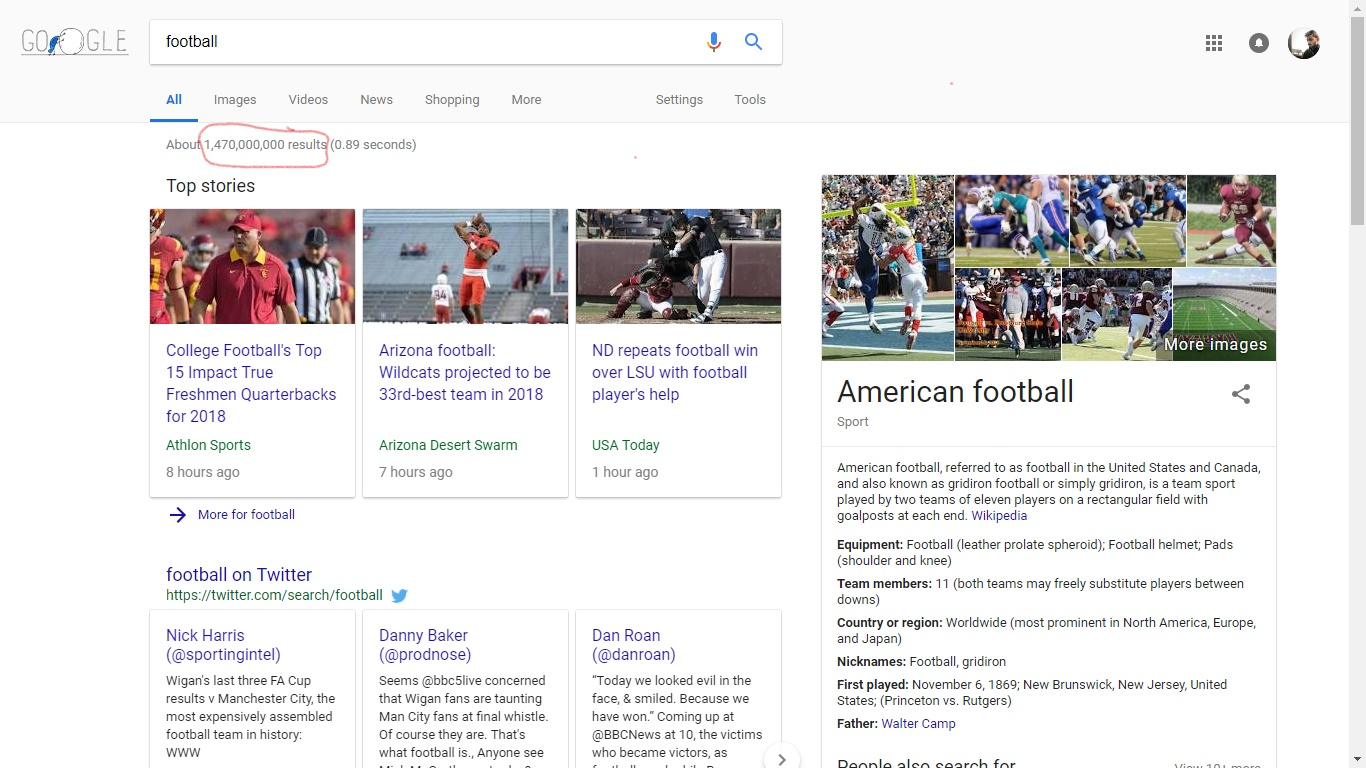
\includegraphics[scale=0.33]{idfDocsTerm.jpg}
\caption{Results from Google query of \emph{football}}
\label{fig:q2cali}
\end{figure}


\begin{table}
\begin{tabular}{ | l | l | l | p{7.8cm} | }
\hline
\textbf{TFIDF} & \textbf{TF} & \textbf{IDF} & \textbf{URI} \\
\hline
0.083 & 0.017 & 4.999 & \url{https://www.azcentral.com/story/sports/high-school/2018/02/08/business-group-trying-keep-valley-junior-college-football-alive-beyond-2018/319131002/?hootPostID=fb32e68c95bcdc943b909439c5c31ba3} \\
\hline
0.074 & 0.015 & 4.999 & \url{http://www.fox26houston.com/news/california-lawmakers-introduce-safe-youth-football-act-by-setting-minimum-age-for-tackle-football?utm_source=dlvr.it&utm_medium=twitter} \\
\hline
0.071 & 0.014 & 4.999 & \url{http://abc7.com/sports/california-bill-would-ban-tackle-football-before-high-school/3058813//} \\
\hline
0.065 & 0.013 & 4.999 & \url{http://www.chicagotribune.com/suburbs/daily-southtown/sports/ct-sta-pat-disabato-column-st-0211-20180209-story.html} \\
\hline
0.035 & 0.007 & 4.999 & \url{http://www.latimes.com/politics/essential/la-pol-ca-essential-politics-updates-california-would-bar-organized-tackle-1518130990-htmlstory.html} \\
\hline
0.023 & 0.005 & 4.999 & \url{http://www.telegram.com/news/20180209/five-st-johns-football-players-among-crop-of-area-athletes-finalizing-college-plans?platform=hootsuite} \\
\hline
0.022 & 0.004 & 4.999 & \url{http://lompocrecord.com/sports/high-school/football/another-taua-to-head-to-reno---this-time/article_a7473c8e-13a8-5f79-82ac-8747900922df.html} \\
\hline
0.021 & 0.039 & 4.999 & \url{http://www.dailymail.co.uk/sport/football/article-5374081/Man-United-star-Mata-fears-football-losing-soul.html?ITO=1490&ns_mchannel=rss&ns_campaign=1490} \\
\hline
0.009 & 0.002 & 4.999 & \url{http://www.bbc.co.uk/sport/football/43010230} \\
\hline
0.006 & 0.001 & 4.999 & \url{http://www.football-chairman.com} \\
\hline
\end{tabular}
\caption{10 URIs found containing football, with calculations TFIDF, TF and IDF}
\label{table:tfidf}
\end{table}






\clearpage

% =================================
% Third question
% =================================

\section*{3}

\subsection*{Question}

\begin{verbatim}
3.  Now rank the same 10 URIs from question #2, but this time 
by their PageRank.  Use any of the free PR estimaters on the web,
such as:

http://pr.eyedomain.com/
http://www.prchecker.info/check_page_rank.php
http://www.seocentro.com/tools/search-engines/pagerank.html
http://www.checkpagerank.net/

If you use these tools, you'll have to do so by hand (they have
anti-bot captchas), but there are only 10 to do.  Normalize the
values they give you to be from 0 to 1.0.  Use the same tool on all
10 (again, consistency is more important than accuracy).  Also
note that these tools typically report on the domain rather than
the page, so it's not entirely accurate.  

Create a table similar to Table 1:

Table 2.  10 hits for the term "shadow", ranked by PageRank.

PageRank	URI
--------	---
0.9		http://bar.com/
0.5		http://foo.com/

Briefly compare and contrast the rankings produced in questions 2
and 3.
\end{verbatim}

\clearpage
\subsection*{Answer}

To calculate the Page Rank for each of the 10 URIs from the previous question I used the \url{http://www.checkpagerank.net/} uri as mentioned in the question. I have stored the values in \textbf{ptdf.csv}. 
 File. Also the values are displayed in the Table \ref{table:pgrank}. First I thought that URIs with high TFIDF values will have higher Page Rank, but this is not the case. From the Table \ref{table:pgrank} we can see that the TFIDF values varies with Page Ranks. Few higher paged rank URIs have lower TFIDF values while a couple of high TFIDF values have lower Page ranks. I have sorted the URIS considering first the Page Rank and then the respective higher TFIDF values since few URIs have the same Page Rank.



\begin{table}
\begin{tabular}{ | l | l | p{8.2cm} | }
\hline
\textbf{Page Rank} & \textbf{TFIDF} & \textbf{URI} \\
\hline
0.9 &  0.0351 & \url{http://www.latimes.com/politics/essential/la-pol-ca-essential-politics-updates-california-would-bar-organized-tackle-1518130990-htmlstory.html} \\
\hline
0.9 & 0.021 & \url{http://www.dailymail.co.uk/sport/football/article-5374081/Man-United-star-Mata-fears-football-losing-soul.html?ITO=1490&ns_mchannel=rss&ns_campaign=1490} \\
\hline
0.9 & 0.009 & \url{http://www.bbc.co.uk/sport/football/43010230} \\
\hline
0.8 & 0.083 & \url{https://www.azcentral.com/story/sports/high-school/2018/02/08/business-group-trying-keep-valley-junior-college-football-alive-beyond-2018/319131002/?hootPostID=fb32e68c95bcdc943b909439c5c31ba3} \\
\hline
0.8 & 0.065 & \url{http://www.chicagotribune.com/suburbs/daily-southtown/sports/ct-sta-pat-disabato-column-st-0211-20180209-story.html} \\
\hline
0.7 & 0.071 & \url{http://abc7.com/sports/california-bill-would-ban-tackle-football-before-high-school/3058813/} \\
\hline
0.7 & 0.023 & \url{http://www.telegram.com/news/20180209/five-st-johns-football-players-among-crop-of-area-athletes-finalizing-college-plans?platform=hootsuite} \\
\hline
0.6 & 0.074 & \url{http://www.fox26houston.com/news/california-lawmakers-introduce-safe-youth-football-act-by-setting-minimum-age-for-tackle-football?utm_source=dlvr.it&utm_medium=twitter} \\
\hline
0.6 & 0.022 & \url{http://lompocrecord.com/sports/high-school/football/another-taua-to-head-to-reno---this-time/article_a7473c8e-13a8-5f79-82ac-8747900922df.html} \\
\hline
0.5 & 0.006 & \url{http://www.football-chairman.com} \\
\hline
\end{tabular}
\caption{Page Rank and TFIDF Comparison of 10 URIs}
\label{table:pgrank}
\end{table}

\clearpage


\section*{4}

\subsection*{Question}

\begin{verbatim}
====================================================
======Question 4 is for 3 points extra credit=======
====================================================

4.  Compute the Kendall Tau_b score for both lists (use "b" because
there will likely be tie values in the rankings).  Report both the
Tau value and the "p" value.

See: 
http://stackoverflow.com/questions/2557863/measures-
of-association-in-r-kendalls-tau-b-and-tau-c
http://en.wikipedia.org/wiki/Kendall_tau_rank_correlation_coefficient#Tau-b
http://en.wikipedia.org/wiki/Correlation_and_dependence
\end{verbatim}

\clearpage
\subsection*{Answer}

For the above problem I first went through \url{http://en.wikipedia.org/wiki/Correlation_and_dependence}
and got to know that it is basically calculating correlaton between pairs of values. The Tau value can have a coefficient between -1 to 1, which means that if the value is 1 or greater it has positive correlation between TFIDF and Page Rank values, meaning they are similar. If the value is zero or close, there is no correlation between them, it’s a tie. And if the value is closer to -1 or less, there is negative correlation, meaning the Page Rank is the opposite of the TFIDF value. Then I went through these references \cite{wikipediaref} and \cite{cranref} and got to know that there is a Kendall package for R language, which gives a summary of values as output. The program reads the TFIDF and Page Rank lists from \textbf{ptdf.csv} file as shown in Listing \ref{lst:q4kendall}.

\lstinputlisting[frame=single,caption={R script to produce summary of Kendall's results },label=lst:q4kendall,captionpos=b,numbers=left,showspaces=false,showstringspaces=false,basicstyle=\footnotesize]{kendall.r}


The summary produced:

\begin{verbatim}
Score =  0 , Var(Score) = 117.4667
denominator =  41.42463
tau = 0, 2-sided pvalue =1

\end{verbatim}

From  the above summary we can see that the tau value is zero meaning there is no correlation between the two pairs of values.

\clearpage


\section*{5}

\subsection*{Question}

\begin{verbatim}
====================================================
======Question 5 is for 3 points extra credit=======
====================================================

5.  Compute a ranking for the 10 URIs from Q2 using Alexa information
(see week 4 slides).  Compute the correlation (as per Q4) for all
pairs of combinations for TFIDF, PR, and Alexa.

\end{verbatim}

\clearpage
\subsection*{Answer}

For the above problem I calculated the Alexa rank from \url{https://www.alexa.com/siteinfo} for each of the 10 URIs which we got in question 2. The values are stored in \textbf{alexa\_rank.csv} file as shown in Table \ref{table:arank}.

\begin{table}
\begin{tabular}{ | l |  p{8.2cm} | }
\hline
\textbf{Alexa Rank} & \textbf{URI} \\
\hline
101 & \url{http://www.bbc.co.uk/sport/football/43010230} \\
\hline
174 & \url{http://www.dailymail.co.uk/sport/football/article-5374081/Man-United-star-Mata-fears-football-losing-soul.html?ITO=1490&ns_mchannel=rss&ns_campaign=1490} \\
\hline
830 & \url{http://www.latimes.com/politics/essential/la-pol-ca-essential-politics-updates-california-would-bar-organized-tackle-1518130990-htmlstory.htm} \\
\hline
2172 & \url{https://www.azcentral.com/story/sports/high-school/2018/02/08/business-group-trying-keep-valley-junior-college-football-alive-beyond-2018/319131002/?hootPostID=fb32e68c95bcdc943b909439c5c31ba3} \\
\hline
7094 & \url{http://www.chicagotribune.com/suburbs/daily-southtown/sports/ct-sta-pat-disabato-column-st-0211-20180209-story.html} \\
\hline
8716 & \url{http://abc7.com/sports/california-bill-would-ban-tackle-football-before-high-school/3058813/} \\
\hline
49281 & \url{http://www.telegram.com/news/20180209/five-st-johns-football-players-among-crop-of-area-athletes-finalizing-college-plans?platform=hootsuite} \\
\hline
125065 & \url{http://www.fox26houston.com/news/california-lawmakers-introduce-safe-youth-football-act-by-setting-minimum-age-for-tackle-football?utm_source=dlvr.it&utm_medium=twitter} \\
\hline
399889 & \url{http://lompocrecord.com/sports/high-school/football/another-taua-to-head-to-reno---this-time/article_a7473c8e-13a8-5f79-82ac-8747900922df.html} \\
\hline
6633445 & \url{http://www.football-chairman.com} \\
\hline
\end{tabular}
\caption{Alexa Rank for 10 URIs}
\label{table:arank}
\end{table}

I calculated the correlation for each of the TFIDF, PR and Alexa values as per Kendall Tau\_b score from question 4. The program is written in R as shown in Listing \ref{lst:q5alexr}. The values are rad from \textbf{alex.r csv} file It produced some interesting results.


\lstinputlisting[frame=single,caption={R program to produe summary of Kendall results},label=lst:q5alexr,captionpos=b,numbers=left,showspaces=false,showstringspaces=false,basicstyle=\footnotesize]{alex.r}

Summary produced for TFIDF and Alexa lists:

\begin{verbatim}
Score =  2 , Var(Score) = 124
denominator =  44.49719
tau = 0.0449, 2-sided pvalue =0.92844
\end{verbatim}

From the above results we can see that the tau value is positive meaning there is some correlation between them, although I thought it would be zero.

Summary produced for Page Rank and Alexa lists:

\begin{verbatim}
Score =  -39 , Var(Score) = 118.3333
denominator =  41.89272
tau = -0.931, 2-sided pvalue =0.00047717

\end{verbatim}

From seeing the above results, I was amazed to see that the Tau\_b value is negative and closer to -1 meaning there is negative correlation between the values, although I thought it would be positive. But then I realized that Alexa scores the URIs opposite to that of the Page Rank, which means that there is correlation and similarity between them.

The correlation between TFIDF and Page Rank has already been tested in question 4.


\clearpage

\section*{6}

\subsection*{Question}

\begin{verbatim}
====================================================
======Question 6 is for 2 points extra credit=======
====================================================

6.  Give an in-depth analysis, complete with examples, 
graphs, and all other pertinent argumentation for 
Kristen Stewart's (of "Twilight" fame) Erdos-Bacon number.

\end{verbatim}

\clearpage
\subsection*{Answer}

The Erdos-Bacon number is nothing but the sum of Erdos number and Bacon number.
To get the Bacon number for Kristen Stewart I visited the \url{https://oracleofbacon.org/movielinks.php} uri which gave me a Bacon number of 2 for Kristen as shown in Figure \ref{fig:q6bacon}.


\begin{figure}[h]
\centering
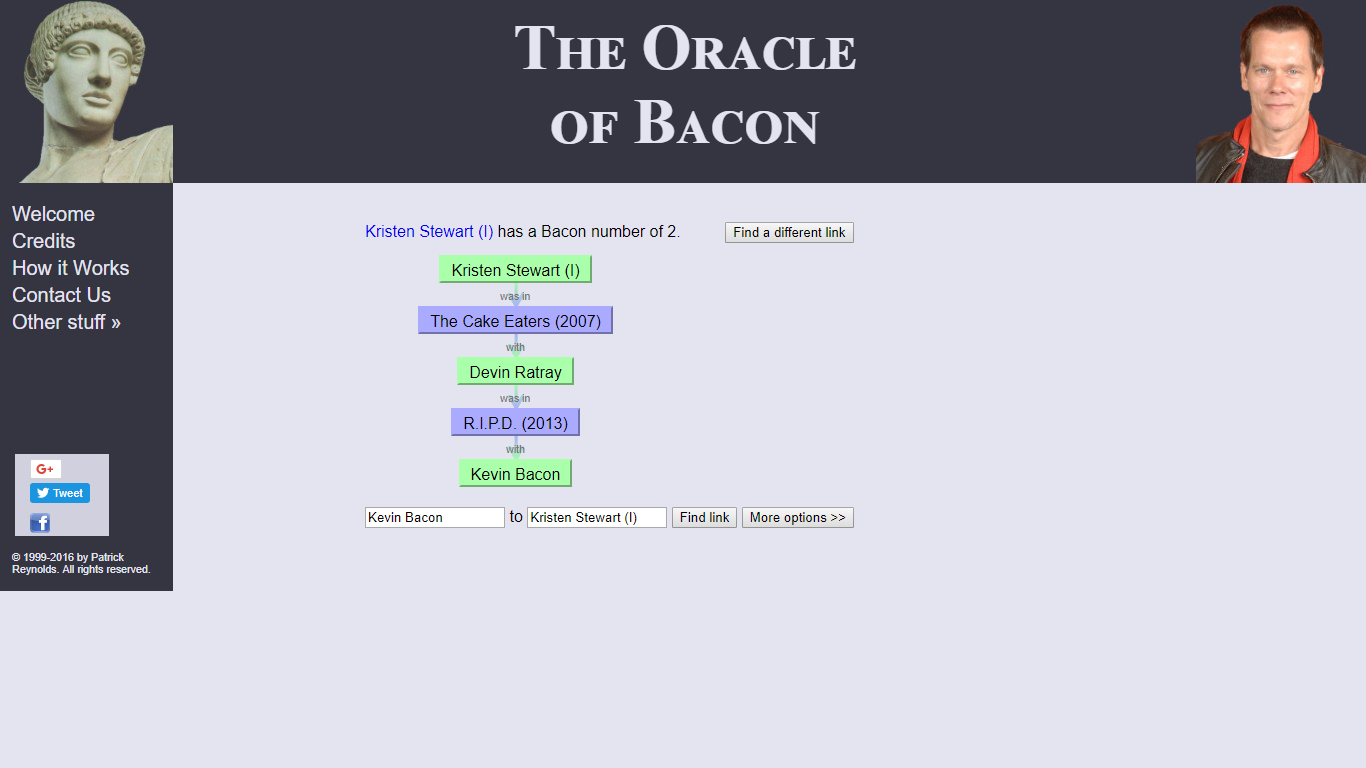
\includegraphics[scale=0.3]{bacon.png}
\caption{Bacon number for Kristen Stewart}
\label{fig:q6bacon}
\end{figure}



To find out the Erdos number for Kristen Stewart I searched through google to know the name of the paper she co-authored. I got to know that she published a paper on machine learning: \url{https://arxiv.org/pdf/1701.04928v1.pdf} along with Bhautik Joshi and David Shapiro. Then on further googling, I encountered a link\url{https://news.ycombinator.com/item?id=13446478} where I came to know that Bhautik Joshi had co-authored in \emph{A quantitative assessment of approaches to mesh generation for surgical simulation} along with Sebastein Ourselin who has a Erdos number of 4 calculated from \url{https://zbmath.org/collaboration-distance/?a=ourselin.sebastien&b=erdos.paul} as shown in Figure\ref{fig:q6erdos}. 

\clearpage

\begin{figure}[h]
\centering
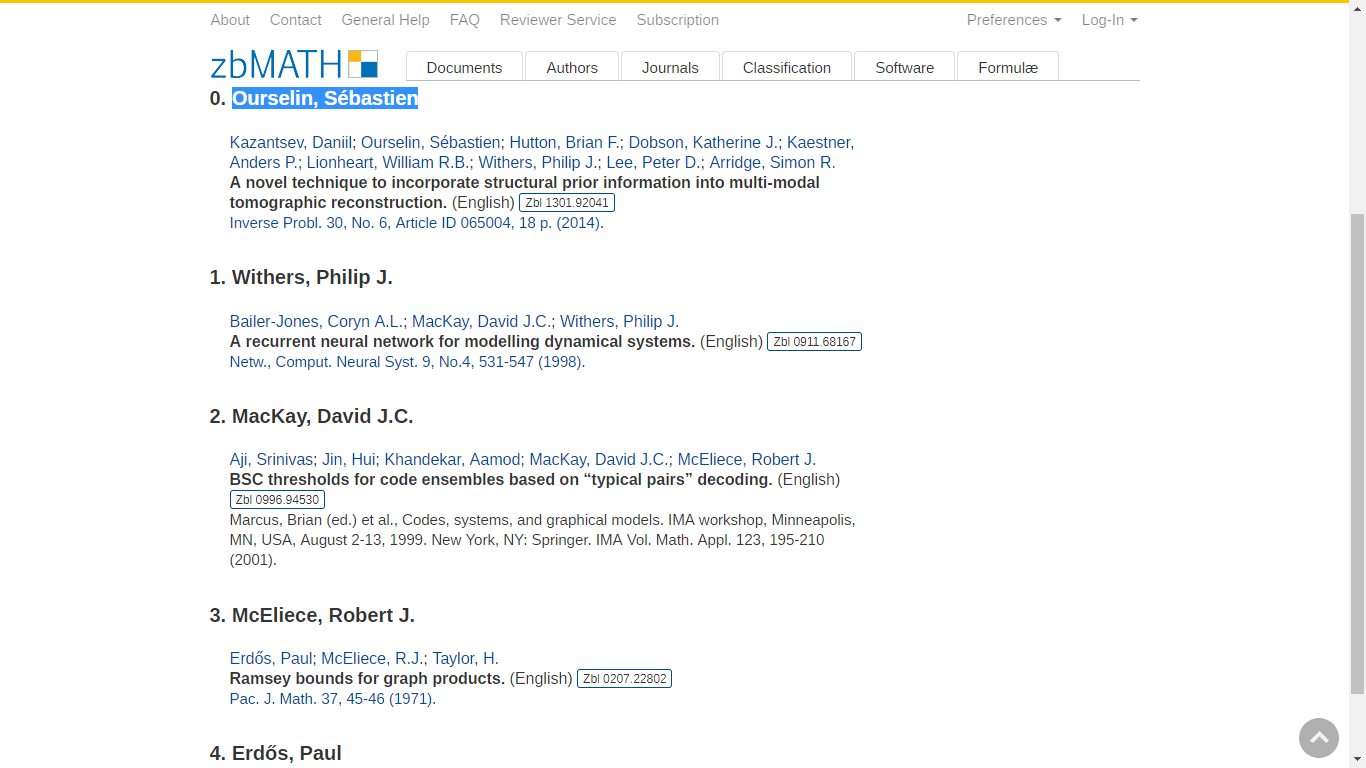
\includegraphics[scale=0.3]{erdos.png}
\caption{Erdos number for Sebastein Ourselin}
\label{fig:q6erdos}
\end{figure}


The following graph was produced using \url{Webgraphviz.com}:


\begin{figure}[h]
\centering

\includegraphics[scale=0.65]{1graph.png}
\caption{Step1: Erdos graph for Kristen Stewart}
\label{fig:q6graphviz}
\end{figure}


\begin{figure}[h]
\centering
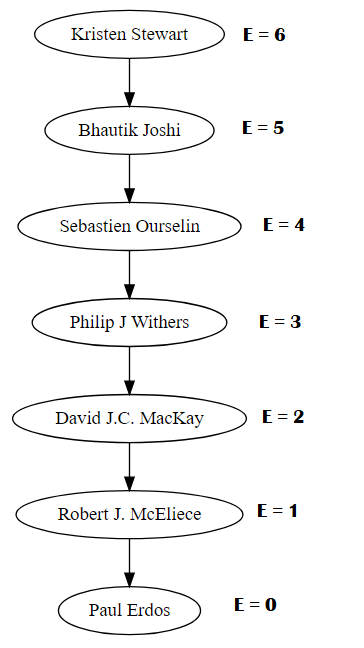
\includegraphics[scale=0.65]{2graph.png}
\caption{Step2: Erdos graph for Kristen Stewart}
\label{fig:q62graphviz}
\end{figure}

From the graph we get the Erdos number for Kristen Stewart as 6. Thus the Erdos-Bacon number for Kristen Stewart is 6 + 2 = 8.

\clearpage



\section*{7}

\subsection*{Question}

\begin{verbatim}
====================================================
======Question 7 is for 2 points extra credit=======
====================================================

7.  Build a simple (i.e., no positional information) inverted file
(in ASCII) for all the words from your 1000 URIs.  Upload the entire
file to github and discuss an interesting portion of the file in
your report.
\end{verbatim}

\clearpage
\subsection*{Answer}

For the above problem which I found very interesting, wrote a program in Python 3.5 as shown in Listing \ref{lst:q7inverted}. First I tested on few of the processed documents from question 1 and created wordlist for each of the document using \emph{obj}.split() \cite{countingref}. I observed that few of the documents had html content which was appending non-linguistic words to the list. I realized that I had to use a different boilerplate removal library, so I went through the \cite{boilerpiperef} and figured out JusText \cite{githubref} is perfect for this. The following dependencies were used:

\begin{itemize}
    \item import justext
    \item import re

\end{itemize}


\lstinputlisting[frame=single,caption={Python script to create an inverted index},label=lst:q7inverted,captionpos=b,numbers=left,showspaces=false,showstringspaces=false,basicstyle=\footnotesize]{read.py}


The program first reads the html documents one by one from the raw\_html folder which we got from question 1 and reads the contents into justext.justext() \cite{githubref} function. It then extracts words using paragraph.text \cite{githubref}. Then it filters all non-alphanumeric characters from the list using re.sub() \cite{regularref}. Then appending the words one by one as key to a dictionary with values as the document number it  writes the output in \textbf{invertedindex.txt} file. A sample output is shown below. What we can see that it starts from document 2 because document 1 had no content.


\begin{figure}[h]
\centering
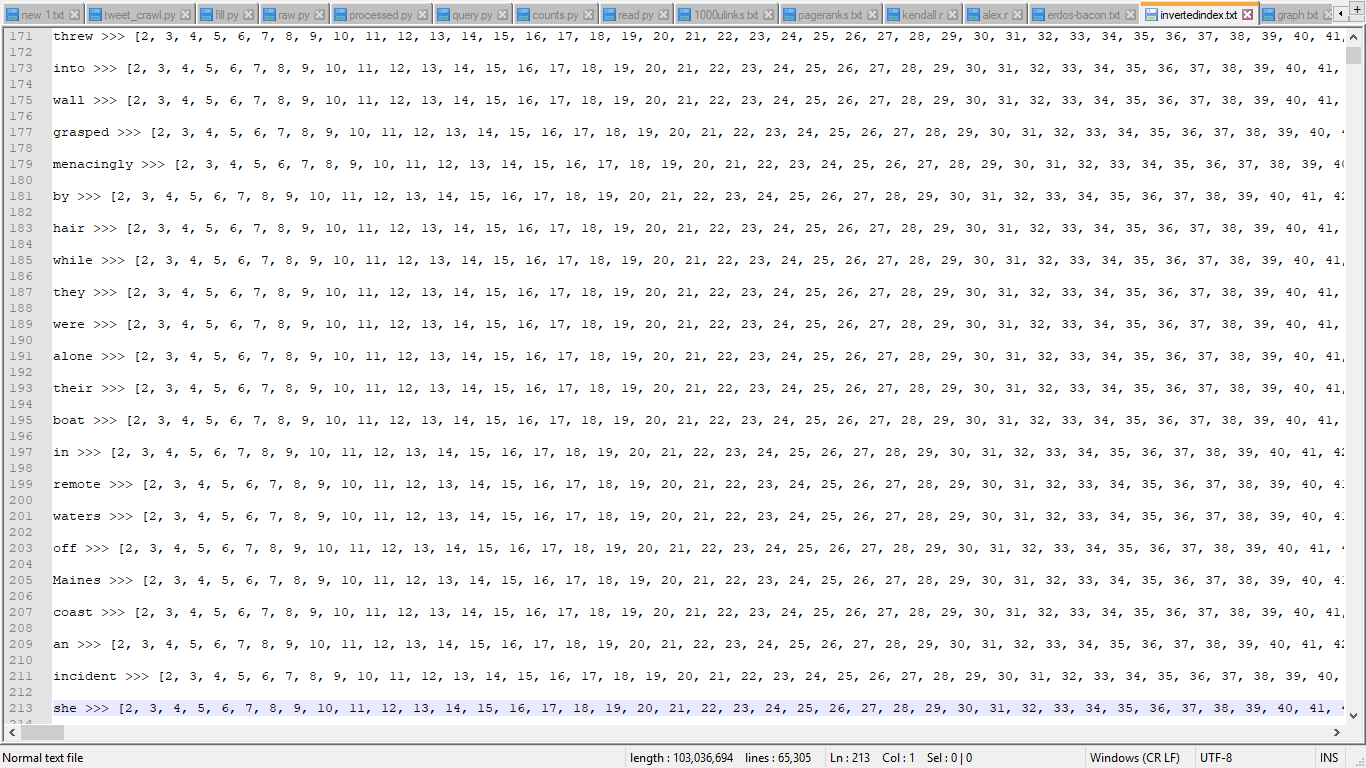
\includegraphics[scale=0.3]{Index.png}
\caption{Inverted Index Output}
\label{fig:q7emojis}
\end{figure}


\clearpage
% =================================
% Bibliography
% =================================

\begin{thebibliography}{9}
\bibitem{requestref}
``Requests: HTTP for Humans.'' equests: HTTP for Humans - Requests 2.18.4 documentation, n.d. Web. February 20, 2018. \url{http://docs.python-requests.org/en/master/}.
\bibitem{unicoderef}
``Stack Overflow.''Switching to Python 3 causing UnicodeDecodeError. N.p.,n.d. Web. February 20, 2018. \url{https://stackoverflow.com/questions/23917729/switching-to-python-3-causing-unicodedecodeerror}
\bibitem{wikipediaref}
``Kendall rank correlation coefficient.'' Wikipedia - Kendall Rank Correlation coefficient. Wikipedia, n.d. Web. February 20, 2018. \url{https://en.wikipedia.org/wiki/Kendall_rank_correlation_coefficient#Tau-b}
\bibitem{cranref}
``CRAN - Package Kendall.''  Kendall Rank Correlation.  n.d. Web. February 20, 2018. \url{https://cran.r-project.org/web/packages/Kendall/Kendall.pdf}
\bibitem{boilerpiperef}
Alexander Nwala. ``Web Science and Digital Libraries Research .'' 2017-03-20: A survey of 5 boilerplate removal methods. N.p., Web. February 20, 2018. \url{http://ws-dl.blogspot.com/2017/03/2017-03-20-survey-of-5-boilerplate.html}.
\bibitem{githubref}
Miso-belica. ``miso-belica/jusText .'',  GitHub,  March 05, 2017, n.d., Web. February 20, 2018. \url{https://github.com/miso-belica/jusText}.
\bibitem{gitref}
Misja. ``misja/python-boilerpipe.'' Github Repository. N.p., October 03, 2017. Web. February 20, 2018.\url{https://github.com/misja/python-boilerpipe}.
\bibitem{regularref}
``6.2. re - Regular expression operations.'' 6.2. re - Regular expression operations - Python 3.6.4 documentation. n.d.,  Web. February 20, 2018. \url{https://docs.python.org/3/library/re.html}.
\bibitem{countingref}
William Turkel-Adam Crymble. ``Counting Word Frequencies with Python'' Programming Historian. N.p., n.d. Web. February 20, 2018.\url{https://programminghistorian.org/lessons/counting-frequencies}.
\bibitem{mathref} 
``9.2. math - Mathematical functions.'' 9.2. math - Mathematical functions - Python 2.7.14 documentation. N.p., n.d. Web. February 20, 2018. \url{https://docs.python.org/2/library/math.html}.
\end{thebibliography}

\end{document}